\subsection{Distributed Memory Model}
\sciwms{} stores data topology locally and fetches numerical
attributes hosted externally from the federation for rendering. Given
a request for a visualization of an attribute regarding a certain
region of interest, the visualization pipeline consists of first
computing the sample locations withing the region of interest, using
the implicit representation for \cgrid{} and \rtree{} for \ugrid{}
topologies, then fetching the external attributes via \ogc{}
web-services. For rendering the sample connectivity within the area of
interest is constructed from the connectivity array which is used for
interpolation. 

The local topology cache and external attribute mechanism defines a
distributed memory model for datasets registered with \sciwms{}
visualized by figure~\ref{fig:sciwms_mem_model}. The grid on the left,
depicts a regular grid stored locally to \sciwms{}. A possible region
of interest is enclosed in the red, dashed square. Attributes are
stored externally by the federations members and are exposed to
\sciwms{} in such a way as it can be visualized by the table on the
left of the figure. Different attribute layers are represented by the
rows of the table while columns correspond to sample locations defined
by the topology. Given the request for a view of an attribute
layer(s), \sciwms{} dispatches a request for the data associated data.

\begin{figure}[ht!]
  \centering
  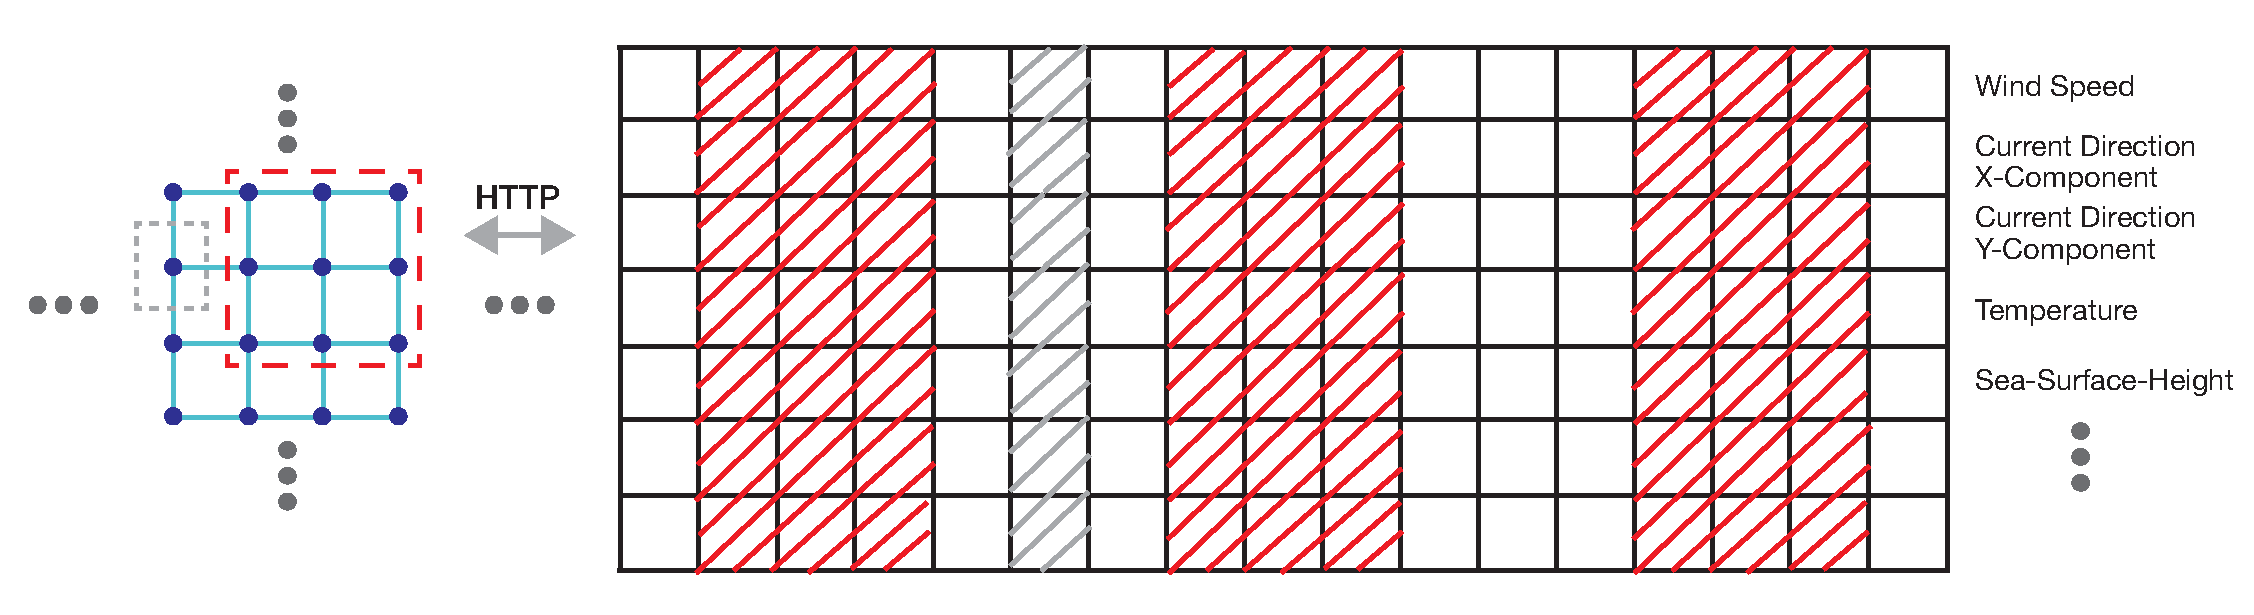
\includegraphics[width=\textwidth]{../figs/topology_memModel}
  \caption{\sciwms{} distributed memory model.}
  \label{fig:sciwms_mem_model}
\end{figure}
